\documentclass[crop,tikz,10pt]{standalone}
\usepackage{tikz}
	\usetikzlibrary{shapes}
	\usetikzlibrary{automata}
	\usetikzlibrary{arrows}
	\usetikzlibrary{backgrounds}
	\usetikzlibrary{calc}
	\usetikzlibrary{positioning}
	\usetikzlibrary{patterns}
	\usetikzlibrary{decorations.pathmorphing}
	\usetikzlibrary{decorations.pathreplacing}

\usepackage[scaled]{helvet}
\renewcommand{\familydefault}{\sfdefault}

\usepackage{siunitx}
\usepackage{booktabs}

\input{../../../../resources/latex/_symbols.qmd}

\begin{document}


\newcommand{\n}[1]{\begin{tabular}{c}#1\end{tabular}}

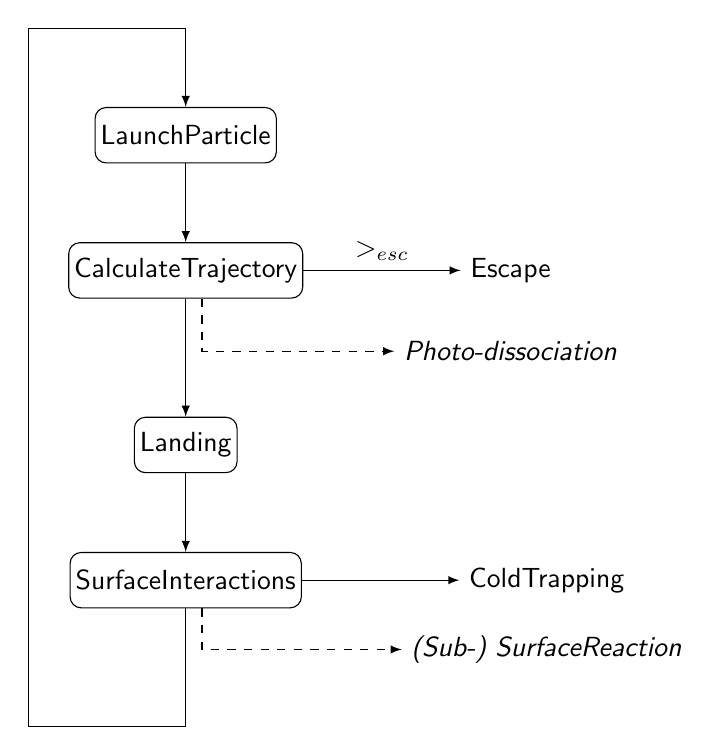
\begin{tikzpicture}[
    main/.style={draw, rounded corners=4pt, inner sep=2pt, minimum size=20pt, minimum width=25pt, fill=white},
    sub/.style={draw, rounded corners=4pt, inner sep=2pt},
]
  
    %::. main nodes
    \node[main] (LAUNCH) at (0,0) {\n{Launch\\ Particle}};
    \node[main, below = of LAUNCH] (TRAJECTORY) {\n{Calculate\\ Trajectory}};
    \node[main, below = 1.5 of TRAJECTORY] (LAND) {\n{Landing}};
    \node[main, below = of LAND] (SURF) {\n{Surface \\ Interactions}};

    %::. main connections
    \draw[-latex] (LAUNCH.270) -- (TRAJECTORY.90);
    \draw[-latex] (TRAJECTORY.270) -- (LAND.90);
    \draw[-latex] (LAND.270) -- (SURF.90);
    \draw[-latex] (SURF.270) |- +(-2,-1.5) -- ($(LAUNCH.90)+(-2,1)$) -| (LAUNCH.90);

    %::. loss nodes
    \node[right = 2 of TRAJECTORY] (ESCAPE) {\n{Escape}};
    \node[right = 2 of SURF] (TRAP) {\n{Cold \\ Trapping}};

    %::. loss connections
    \draw[-latex] (TRAJECTORY) -- (ESCAPE) node [midway, above] {$\velocity > \velocity_{esc}$ };
    \draw[-latex] (SURF) -- (TRAP);

    %::. conversion nodes
    \node[below = 0.5 of ESCAPE] (PHOTO) {\textit{\n{Photo- \\ dissociation}}};
    \node[below = 0.3 of TRAP] (CONV) {\textit{\n{(Sub-) Surface \\ Reaction}}};

    %::. conversion connections
    \draw[-latex, dashed] (TRAJECTORY.300) |- (PHOTO);
    \draw[-latex, dashed] (SURF.300) |- (CONV);
\end{tikzpicture}

\end{document}